\documentclass[12pt,a4paper]{article}

% Packages
\usepackage{graphicx}   % for including figures
\usepackage{booktabs}   % for nice tables
\usepackage{hyperref}   % for clickable links
\usepackage{float}      % for [H] placement of figures/tables
\usepackage{caption}
\usepackage{subcaption}
\usepackage{multirow}

\title{COS226 Assignment 1}
\author{Dewald Colesky u23536030}
\date{\today}

\begin{document}

\maketitle

\section{Introduction}
In this report we evaluate the performance and fairness of TTAS and CLH locks under different contention levels (LOW, MEDIUM, HIGH) and player counts (2, 8, 16).

\clearpage
\section{Results}


\subsection{Execution Time Graphs}
Figure~\ref{fig:execution-time} shows the execution time as the number of players increases.

\begin{figure}[H]
  \centering
  % Top row: Low and Medium contention side by side
  \begin{subfigure}{0.48\textwidth}
    \centering
    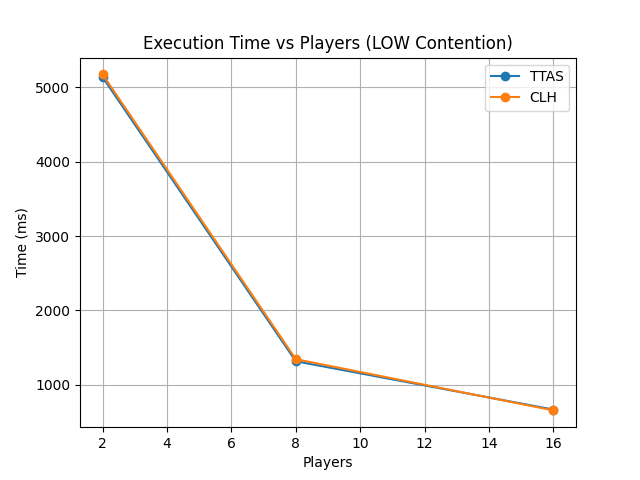
\includegraphics[width=\linewidth]{plot_time_LOW.png}
    \caption{Low contention}
    \label{fig:time-low}
  \end{subfigure}
  \hfill
  \begin{subfigure}{0.48\textwidth}
    \centering
    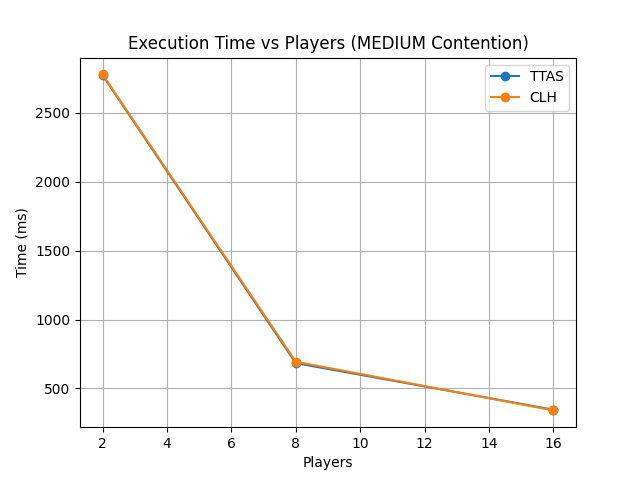
\includegraphics[width=\linewidth]{plot_time_MEDIUM.png}
    \caption{Medium contention}
    \label{fig:time-med}
  \end{subfigure}
  
  % Bottom row: High contention full width
  \vspace{0.5em}
  \begin{subfigure}{0.65\textwidth}
    \centering
    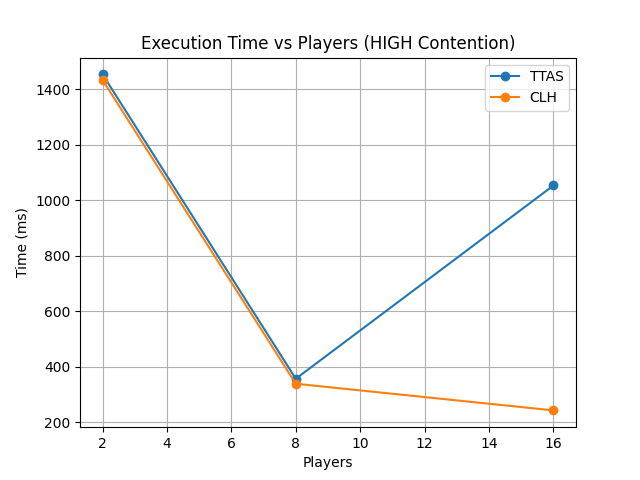
\includegraphics[width=\linewidth]{plot_time_HIGH.png}
    \caption{High contention}
    \label{fig:time-high}
  \end{subfigure}
  
  \caption{Execution time as the number of players increases. Subfigures (a), (b), and (c) correspond to Low, Medium, and High contention respectively.}
  \label{fig:execution-time}
\end{figure}
  
\clearpage
\subsection{Execution Time Discussion}
Low and medium contention has largely similiar results, with execution time being nearly identical regardless of the amount of players. This result will be discussed in detail.
High contention has similiar execution for 2 and 8 players however at 16 players the difference in these locks reallt shows. CLH is almost 4 time faster than TTAS and this is because CLH avoids busy spinning on the shared lock because each thread spins on a local variable which reduces cache coherence traffic.

For low and medium contention there simply isn't enough contention for
 either. This is mainly because of modern CPU's and thread optimization. This leads to execution-time being almost entirely determined by work inside the critical section. Hence the similiar execution-time until the lock becomes the bottleneck at high contention. See below a graph where think time is constant (5ms) and work time is (1 000, 100 000, 1 000 000) for low, medium, and high contention respectively.

As seen in Figure~\ref{fig:execution-time-const} , the results are still largely the same with slight differences. This can differ on a machine with less threads or by using much greater work time.

\begin{figure}[H]
  \centering
  % Top row: Low and Medium contention side by side
  \begin{subfigure}{0.48\textwidth}
    \centering
    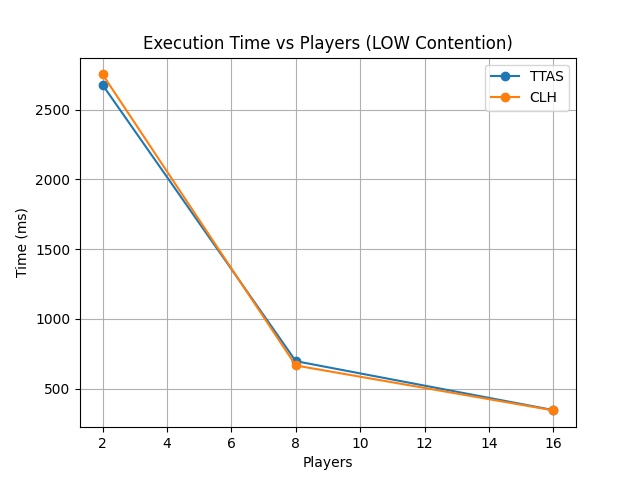
\includegraphics[width=\linewidth]{const_plot_time_LOW.png}
    \caption{Low contention}
    \label{fig:const-time-low}
  \end{subfigure}
  \hfill
  \begin{subfigure}{0.48\textwidth}
    \centering
    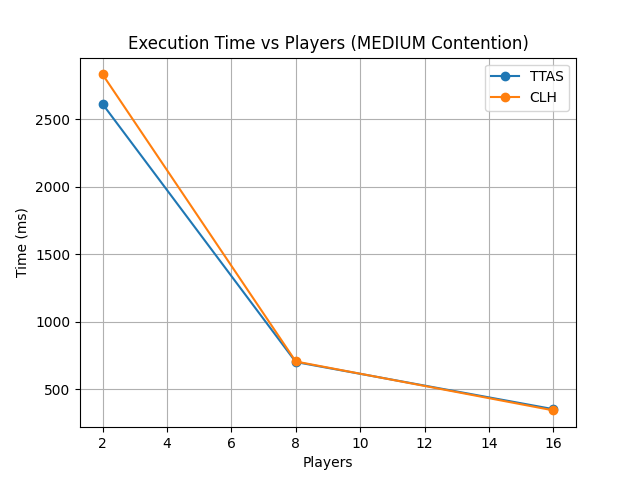
\includegraphics[width=\linewidth]{const_plot_time_MEDIUM.png}
    \caption{Medium contention}
    \label{fig:const-time-med}
  \end{subfigure}
  
  % Bottom row: High contention full width
  \vspace{0.5em}
  \begin{subfigure}{0.65\textwidth}
    \centering
    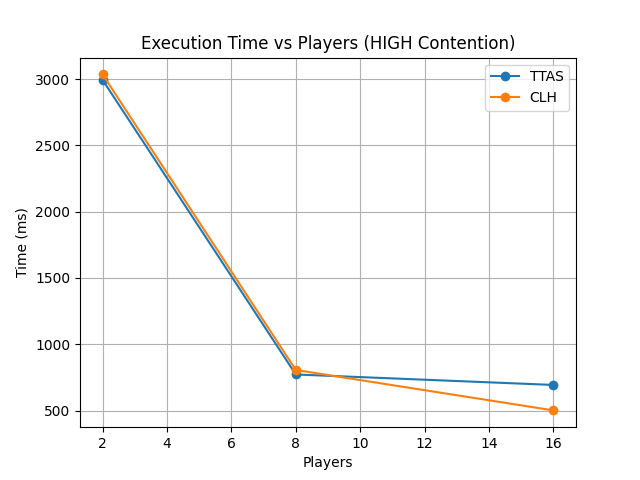
\includegraphics[width=\linewidth]{const_plot_time_HIGH.png}
    \caption{High contention}
    \label{fig:const-time-high}
  \end{subfigure}
  
    \caption{Execution time as the number of players increases (with constant think time). Subfigures (a), (b), and (c) correspond to Low, Medium, and High contention respectively.}
  \label{fig:execution-time-const}
\end{figure}

\clearpage
\subsection{Fairness Table}
Table~\ref{tab:fairness} compares the fairness spread (Max--Min coins taken).

\begin{table}[H]
\centering
\begin{tabular}{@{}llcccc@{}}
\toprule
Lock & Players & Contention & Min & Max & Spread \\ \midrule
\multirow{9}{*}{TTAS}
    & 2  & LOW    & 979  & 1021 & 42  \\
    & 2  & MED    & 988  & 1012 & 24  \\
    & 2  & HIGH   & 999  & 1001 & 2   \\
    & 8  & LOW    & 235  & 261  & 26  \\
    & 8  & MED    & 239  & 263  & 24  \\
    & 8  & HIGH   & 228  & 263  & 35  \\
    & 16 & LOW    & 114  & 138  & 24  \\
    & 16 & MED    & 113  & 139  & 26  \\
    & 16 & HIGH   & 77   & 163  & 86  \\ \midrule
\multirow{9}{*}{CLH}
    & 2  & LOW    & 977  & 1023 & 46  \\
    & 2  & MED    & 992  & 1008 & 16  \\
    & 2  & HIGH   & 998  & 1002 & 4   \\
    & 8  & LOW    & 236  & 260  & 24  \\
    & 8  & MED    & 233  & 259  & 26  \\
    & 8  & HIGH   & 233  & 263  & 30  \\
    & 16 & LOW    & 113  & 132  & 19  \\
    & 16 & MED    & 115  & 133  & 18  \\
    & 16 & HIGH   & 113  & 135  & 22  \\ 
\bottomrule
\end{tabular}

\caption{Fairness comparison (Min--Max coins taken and Spread) between TTAS and CLH locks across players and contention levels.}
\label{tab:fairness}
\end{table}

\clearpage
\subsection{Fairness Graphs}
Figure~\ref{fig:fairness-plots} shows the fairness as the number of players increases.

\begin{figure}[H]
  \centering
  % Top row: Low and Medium contention side by side
  \begin{subfigure}{0.48\textwidth}
    \centering
    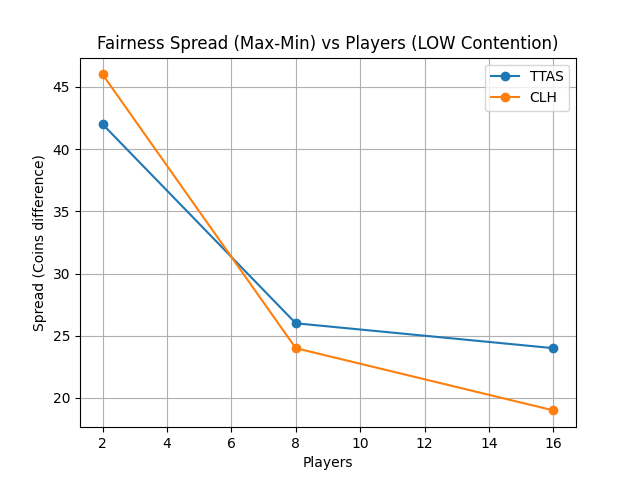
\includegraphics[width=\linewidth]{plot_fairness_LOW.png}
    \caption{Low contention}
    \label{fig:fairness-low}
  \end{subfigure}
  \hfill
  \begin{subfigure}{0.48\textwidth}
    \centering
    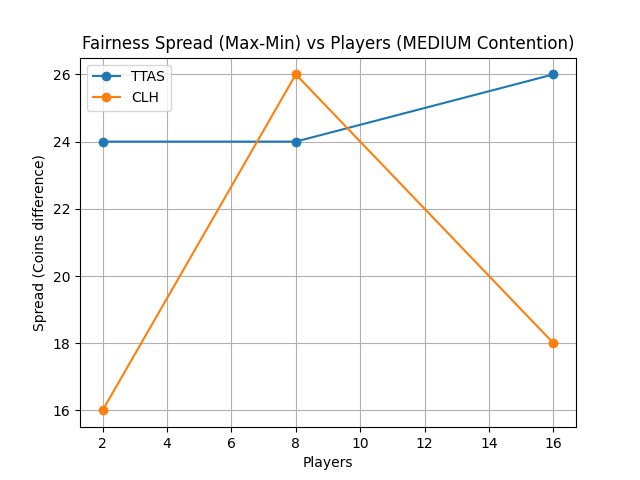
\includegraphics[width=\linewidth]{plot_fairness_MEDIUM.png}
    \caption{Medium contention}
    \label{fig:fairness-med}
  \end{subfigure}
  
  % Bottom row: High contention full width
  \vspace{0.5em}
  \begin{subfigure}{0.65\textwidth}
    \centering
    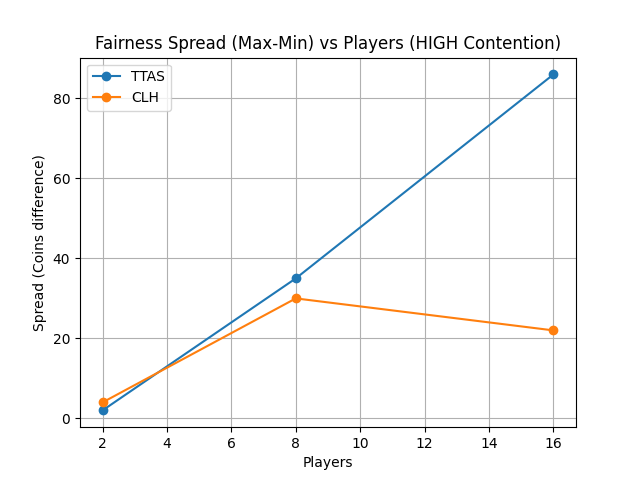
\includegraphics[width=\linewidth]{plot_fairness_HIGH.png}
    \caption{High contention}
    \label{fig:fairness-high}
  \end{subfigure}
  
  \caption{Fairness as the number of players increases. Subfigures (a), (b), and (c) correspond to Low, Medium, and High contention respectively.}
  \label{fig:fairness-plots}
\end{figure}

\clearpage
\subsection{Fairness Discussion}
The fairness measured is how evenly threads acquire the lock and take resources from the treasure chest.

Under low contention, both TTAS and CLH exhibit relatively small spreads because threads don't often block eachother.

Under medium contention the difference appears with CLH generally maining a lower spread than TTAS. Although with 8 players the difference is larger for CLH - but still relatively similiar to TTAS.

Under high contention there is a clear distinction. CLH consistently provides lower spread (with results varying slightly from run to run). This is becuase CLH provides more uniform access while TTAS can favour certain threads and uses a shared variable for spinning. CLH uses a queue-based design for a roughly FIFO order which reduces contention-related spread.


\clearpage
\section{Final Comparison}
Both locks will provide similiar performance with low contention (2, 8 players and Low, Medium conention). The difference appears when the lock is under a lock of contention, this allows CLH's queue-based design to outperform TTAS in both execution-time and fairness by large margins. TTAS may favour certain threads and skew fairness thus TTAS should only be used in simpler, and predictable environments where threads don't do extreme work in critical sections. 

\section{Conclusion}
CLH demonstrates better fairness as contention and thread count increase, while TTAS can lead to uneven distribution under heavy load and should be used in predictable environments.



All data and source code for this report are available on github under `A1`. 
Visit \href{https://github.com/amJohnnyma/COS226.git}{GitHub} for all graphs and source code.


\end{document}
